\documentclass[12pt]{article}

%%%%%%%%%%%%%%%%%%%%%%%%%%%%%%%%%%%%%%%%%%%%%%%%%%%%%%%%%%%%%%%%%%%%%%%%%%%%%%%%
%                           Package preset for homework
%%%%%%%%%%%%%%%%%%%%%%%%%%%%%%%%%%%%%%%%%%%%%%%%%%%%%%%%%%%%%%%%%%%%%%%%%%%%%%%%
% Miscellaneous
\usepackage[margin=1in]{geometry}
\usepackage[utf8]{inputenc}
\usepackage{indentfirst}
\usepackage{blindtext}
\usepackage{graphicx}
\usepackage{xr-hyper}
\usepackage{hyperref}
\usepackage{enumitem}
\usepackage{color}
\usepackage{float}
% Math
\usepackage{latexsym}
\usepackage{amsfonts}
\usepackage{amssymb}
\usepackage{amsmath}
\usepackage{commath}
\usepackage{amsthm}
\usepackage{bbold}
\usepackage{bm}
% Physics
\usepackage{physics}
\usepackage{siunitx}
% Code typesetting
\usepackage{listings}
% Citation
\usepackage[authoryear]{natbib}
\usepackage{appendix}
\usepackage[capitalize]{cleveref}
% Title & name
\title{Homework}
\author{Tien Vo}
\date{\today}


%%%%%%%%%%%%%%%%%%%%%%%%%%%%%%%%%%%%%%%%%%%%%%%%%%%%%%%%%%%%%%%%%%%%%%%%%%%%%%%%
%                   User-defined commands and environments
%%%%%%%%%%%%%%%%%%%%%%%%%%%%%%%%%%%%%%%%%%%%%%%%%%%%%%%%%%%%%%%%%%%%%%%%%%%%%%%%
%%% Misc
\sisetup{load-configurations=abbreviations}
\newcommand{\due}[1]{\date{Due: #1}}
\newcommand{\hint}{\textit{Hint}}
\let\oldt\t
\renewcommand{\t}[1]{\text{#1}}

%%% Bold sets & abbrv
\newcommand{\N}{\mathbb{N}}
\newcommand{\Z}{\mathbb{Z}}
\newcommand{\R}{\mathbb{R}}
\newcommand{\Q}{\mathbb{Q}}
\let\oldP\P
\renewcommand{\P}{\mathbb{P}}
\newcommand{\LL}{\mathcal{L}}
\newcommand{\FF}{\mathcal{F}}
\newcommand{\HH}{\mathcal{H}}
\newcommand{\NN}{\mathcal{N}}
\newcommand{\ZZ}{\mathcal{Z}}
\newcommand{\RN}[1]{\textup{\uppercase\expandafter{\romannumeral#1}}}
\newcommand{\ua}{\uparrow}
\newcommand{\da}{\downarrow}

%%% Unit vectors
\newcommand{\xhat}{\vb{\hat{x}}}
\newcommand{\yhat}{\vb{\hat{y}}}
\newcommand{\zhat}{\vb{\hat{z}}}
\newcommand{\nhat}{\vb{\hat{n}}}
\newcommand{\rhat}{\vb{\hat{r}}}
\newcommand{\phihat}{\bm{\hat{\phi}}}
\newcommand{\thetahat}{\bm{\hat{\theta}}}

%%% Other math stuff
\providecommand{\units}[1]{\,\ensuremath{\mathrm{#1}}\xspace}
% Set new style for problem
\newtheoremstyle{problemstyle}  % <name>
        {10pt}                   % <space above>
        {10pt}                   % <space below>
        {\normalfont}           % <body font>
        {}                      % <indent amount}
        {\bfseries\itshape}     % <theorem head font>
        {\normalfont\bfseries:} % <punctuation after theorem head>
        {.5em}                  % <space after theorem head>
        {}                      % <theorem head spec (can be left empty, 
                                % meaning `normal')>

% Set problem environment
\theoremstyle{problemstyle}
\newtheorem{problemenv}{Problem}[section]
\newenvironment{problem}[1]{%
  \renewcommand\theproblemenv{#1}%
  \problemenv
}{\endproblemenv}
% Set lemma environment
\newenvironment{lemma}[2][Lemma]{\begin{trivlist}
\item[\hskip \labelsep {\bfseries #1}\hskip \labelsep {\bfseries #2.}]}{\end{trivlist}}
% Set solution environment
\newenvironment{solution}{
    \begin{proof}[Solution]$ $\par\nobreak\ignorespaces
}{\end{proof}}
\numberwithin{equation}{problemenv}

%%% Page format
\setlength{\parindent}{0.5cm}
\setlength{\oddsidemargin}{0in}
\setlength{\textwidth}{6.5in}
\setlength{\textheight}{8.8in}
\setlength{\topmargin}{0in}
\setlength{\headheight}{18pt}

%%% Code environments
\definecolor{dkgreen}{rgb}{0,0.6,0}
\definecolor{gray}{rgb}{0.5,0.5,0.5}
\definecolor{mauve}{rgb}{0.58,0,0.82}
\lstset{frame=tb,
  language=Python,
  aboveskip=3mm,
  belowskip=3mm,
  showstringspaces=false,
  columns=flexible,
  basicstyle={\small\ttfamily},
  numbers=none,
  numberstyle=\tiny\color{gray},
  keywordstyle=\color{blue},
  commentstyle=\color{dkgreen},
  stringstyle=\color{mauve},
  breaklines=true,
  breakatwhitespace=true,
  tabsize=4
}
\lstset{
  language=Mathematica,
  numbers=left,
  numberstyle=\tiny\color{gray},
  numbersep=5pt,
  breaklines=true,
  captionpos={t},
  frame={lines},
  rulecolor=\color{black},
  framerule=0.5pt,
  columns=flexible,
  tabsize=2
}


\title{Homework 3: Phys 7310 (Fall 2021)}

\begin{document}

\maketitle

%%%%%%%%%%%%%%%%%%%%%%%%%%%%%%%%%%%%%%%%%%%%%%%%%%%%%%%%%%%%%%%%%%%%%%%%%%%%%%%%
\begin{problem}{3.1}[A plate with a half-sphere]~\\
    \begin{figure}[h]
        \centering
        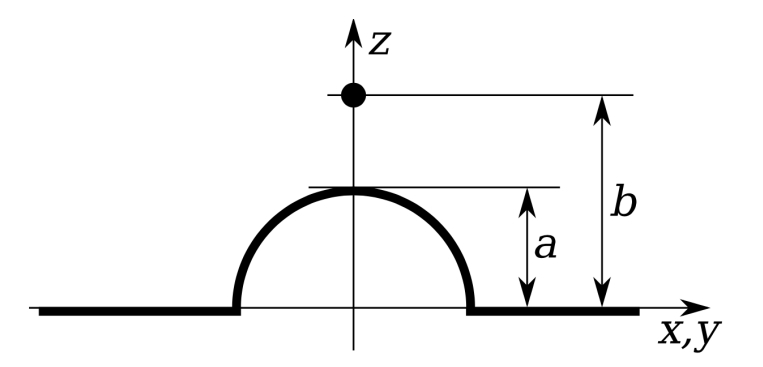
\includegraphics[width=0.5\textwidth]{hw3_p1.jpg}
    \end{figure}
An infinite grounded conducting plate has a bulge in form of a haf-sphere with
radius $a$. A point charge $q$ is put on the symmetry axis of the system at a
distance $b>a$ from the center of the half-sphere (see figure). Using the method
of image, calculate the potential $\Phi$ above the plate, the force on the point
charge $q$, and the total charge induced on the half-sphere.
\begin{solution}
This conductor has both the geometry of (i) the infinite plane conductor 
and (ii) the spherical conductor, already solved in Jackson and in class.
The boundary condition requires that (I) the potential at the infinite plane
($x^2+y^2\geq a^2$) is zero and (II) the potential on the hemisphere
($z=\sqrt{a^2-x^2-y^2}$) is zero.

In (i), there needs an image charge $-q$ placed at $z=-b$ to satisfy (I). In
(ii), an image charge $q'=-(a/b)q$ is placed at $z'=a^2/b$ to satisfy (II).
However, now that there is a second image charge, (I) is no longer satisfied. As
a remedy, there needs a third image charge $-q'=(a/b)q$ at $z=-z'$ so that (I) 
is satisfied. Note that by symmetry, (II) is also satisfied with this third 
image charge (imagine a situation where $-q$ at $z=-b$ is the real charge and 
we have to place a charge $q''=-(a/b)(-q)$ at $z''=-a^2/b$ for the potential at
$\abs{\vb{x}}=a$ to be zero. This applies for both hemispheres, so the
existence of the third image charge does not affect the potential at the bulge).

Now, we can write the total potential as
\begin{align}\label{p1:Phi_cartesian}
    \Phi(\vb{x})
    &=\frac{q}{4\pi\epsilon_0}\Bigg\{
        \qty[x^2+y^2+(z-b)^2]^{-1/2}-\qty[x^2+y^2+(z+b)^2]^{-1/2}\notag\\
    &\qquad+\frac{a}{b}\qty[
            \qty[x^2+y^2+\qty(z+a^2/b)^2]^{-1/2}
            -\qty[x^2+y^2+\qty(z-a^2/b)^2]^{-1/2}
        ]
    \Bigg\}
\end{align}
To verify that this potential is zero at the conductor, we consider two cases:

\textbf{Case 1}: $z=0$ (on the plane conductor)
\begin{align}
    \Phi&\sim\qty[x^2+y^2+b^2]^{-1/2}-\qty[x^2+y^2+b^2]^{-1/2}\notag\\
        &\qquad+\frac{a}{b}\qty[x^2+y^2+a^4/b^2]^{-1/2}
        -\frac{a}{b}\qty[x^2+y^2+a^4/b^2]^{-1/2}\notag\\
        &=0
\end{align}

\textbf{Case 2}: $z=\sqrt{a^2-x^2-y^2}$ (on the spherical bulge)

\begin{align}
    \Phi&\sim\qty[a^2-z^2+(z-b)^2]^{-1/2}-\qty[a^2-z^2+(z+b)^2]^{-1/2}\notag\\
        &\qquad+\frac{a}{b}\qty{
            \qty[a^2-z^2+(z+a^2/b)^2]^{-1/2}-\qty[a^2-z^2+(z-a^2/b)^2]^{-1/2}
        }\notag\\
        &=\qty[a^2-2zb+b^2]^{-1/2}-\qty[a^2+2zb+b^2]^{-1/2}\notag\\
        &\qquad\qty(\frac{b^2}{a^2})^{-1/2}\qty{
            \qty[a^2+2(a^2/b)z+a^4/b^2]^{-1/2}
            -\qty[a^2-2(a^2/b)z+a^4/b^2]^{-1/2}
        }\notag\\
        &=\qty[a^2-2zb+b^2]^{-1/2}-\qty[a^2+2zb+b^2]^{-1/2}
        +\qty[b^2+2zb+a^2]^{-1/2}-\qty[b^2-2zb+a^2]^{-1/2}\notag\\
        &=0
\end{align}

The electric field generated by the three image charges at $z=b$ is
\begin{align}
    \vb{E}&=\frac{q}{4\pi\epsilon_0}\qty{\frac{a}{b}\qty[
        \frac1{(b+a^2/b)^2}
        -\frac1{(b-a^2/b)^2}
        ]
        -\frac1{4b^2}
    }\zhat\notag\\
    &=-\frac{q}{4\pi\epsilon_0}\qty[\frac{4a^3b^3}{(b^4-a^4)^2}+\frac1{4b^2}]\zhat
\end{align}
Thus, the force exerted on the real charge $q$ is
\begin{equation}
    \vb{F}=q\vb{E}=-\frac{q^2}{4\pi\epsilon_0}\qty[\frac{4a^3b^3}{(b^4-a^4)^2}+\frac1{4b^2}]\zhat
\end{equation}

Note that we can rewrite \eqref{p1:Phi_cartesian} in spherical coordinates
\begin{align}
    \Phi(\vb{x})&=\frac{q}{4\pi\epsilon_0}\qty[
        \frac1{\abs{\vb{x}-b\zhat}}-\frac1{\abs{\vb{x}+b\zhat}}
        +\frac{a}{b}\qty(
            \frac{1}{\abs{\vb{x}+(a^2/b)\zhat}}
            -\frac{1}{\abs{\vb{x}-(a^2/b)\zhat}}
        )
    ]\notag\\
    &=\frac{q}{4\pi\epsilon_0}\Bigg\{
        \qty(r^2+b^2-2br\cos\theta)^{-1/2}-(r^2+b^2+2br\cos\theta)^{-1/2}\notag\\
    &\qquad+\frac{a}{b}\qty[
        (r^2+a^4/b^2+2(a^2/b)r\cos\theta)^{-1/2}
        -(r^2+a^4/b^2-2(a^2/b)r\cos\theta)^{-1/2}
    ]
    \Bigg\}
\end{align}
where $\abs{\vb{x}}=r$. With the help of Mathematica, we can find the
directional derivative of $\Phi$ in the direction normal to the spherical bulge
($\partial/\partial n=\partial/\partial r$)
\begin{align}
    \frac{\partial\Phi}{\partial r}&=\frac{q}{4\pi\epsilon_0}\Bigg\{
        \frac{b\cos\theta-r}{(r^2+b^2-2br\cos\theta)^{3/2}}
        +\frac{b\cos\theta+r}{(r^2+b^2+2br\cos\theta)^{3/2}}\notag\\
       &\qquad+\frac{(b^2/a^2)r-b\cos\theta}{(a^2+(b^2/a^2)r^2-2br\cos\theta)^{3/2}}
        -\frac{(b^2/a^2)r+b\cos\theta}{(a^2+(b^2/a^2)r^2+2br\cos\theta)^{3/2}}
    \Bigg\}
\end{align}
The surface charge density at $r=a$ is thus
\begin{equation}
    \sigma=-\epsilon_0\eval{\frac{\partial\Phi}{\partial r}}_{r=a}
    =-\frac{q}{4\pi}\frac{b^2-a^2}{a}\qty[\frac1{(a^2+b^2-2ab\cos\theta)^{3/2}}-\frac1{(a^2+b^2+2ab\cos\theta)^{3/2}}]
\end{equation}
Then we can calculate the total induced charge on the bulge (where
$da=a^2\sin\theta d\theta d\phi$)
\begin{align}
    Q_{\text{induced}}
    &=\int_{\text{bulge}}\sigma da\notag\\
    &=-\frac{q}{2}a(b^2-a^2)\int_0^{\pi/2}\qty[
    \frac1{(a^2+b^2-2ab\cos\theta)}^{3/2}
    -\frac1{(a^2+b^2+2ab\cos\theta)}^{3/2}
    ]\sin\theta d\theta\notag\\
    &=-\frac{q}{4}\frac{b^2-a^2}{b}\qty[\int_{(a-b)^2}^{a^2+b^2}\frac{du_-}{u_-^{3/2}}+\int_{(a+b)^2}^{a^2+b^2}\frac{du_+}{u_+^{3/2}}]\tag{$u_\pm=a^2+b^2\pm2ab\cos\theta$}\\
    &=\frac{q}{2}\frac{b^2-a^2}{b}\qty[\frac{2}{\sqrt{a^2+b^2}}-\frac1{b-a}-\frac{1}{a+b}]\notag\\
    &=\frac{b^2-a^2}{b\sqrt{a^2+b^2}}q-q
\end{align}
\end{solution}
\end{problem}
%%%%%%%%%%%%%%%%%%%%%%%%%%%%%%%%%%%%%%%%%%%%%%%%%%%%%%%%%%%%%%%%%%%%%%%%%%%%%%%%
\begin{problem}{3.2}[A line charge]
In this problem, we consider an infinite line with a constant linear charge
density $\lambda$ (charge per unit length). Let the line charge sit at the
origin $(x,y)=(0,0)$ in the $xy$-plane, and stretch infinitely in both
directions along the $z$-axis.

Draw an appropriate Gaussian surface and find the electric field a distance $r$
away from the line charge. Show that a potential for this electric field takes
the form
\begin{equation}
    \Phi(\vb{x})=\alpha\ln\frac{r}{R} 
\end{equation}
where $\alpha$ is a constant you should determine in terms of $\lambda$ and
other things, and $R$ is a \textit{totally arbitrary} constant with units of
length that we include to make the units in the log dimensionless; explain why
$R$ drops out of physically measurable quantities. Finally, if there is another
line charge with linear charge density $\lambda'$ a distance $r$ away from the
first charge, find the force per unit length experienced by this second line
charge.
\begin{solution}
\begin{center}
    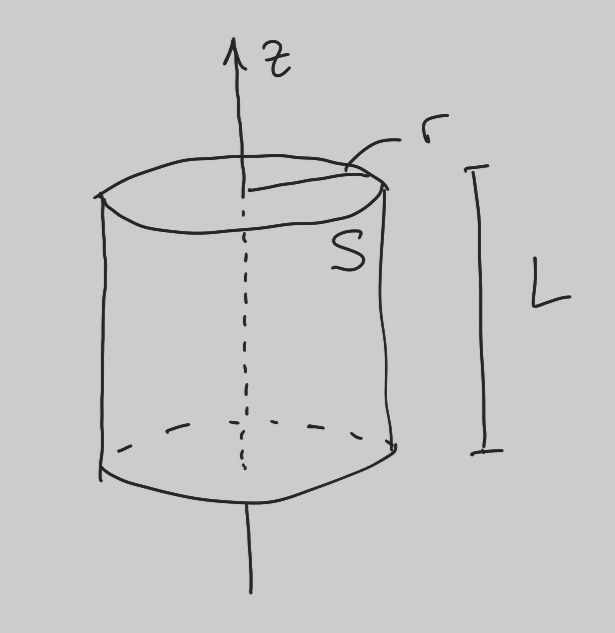
\includegraphics[width=0.5\textwidth]{hw3_p2.jpg} 
\end{center}

Draw a cylindrical Gaussian surface $S$ enclosing the line charge along a
length $L$ as above. By Gauss Law,
\begin{equation}
    \oint_S\vb{E}\vdot\nhat da=E2\pi rL=\frac{\lambda L}{\epsilon_0} 
\end{equation}
Then by symmetry, we can write
\begin{equation}
    \vb{E}=\frac{\lambda}{2\pi\epsilon_0}\frac{1}{r}\rhat 
\end{equation}
By definition, the potential difference between $r=R$ and $r=r$ is then
\begin{equation}
    \Phi(r)-\Phi(R)=-\int_R^r\vb{E}\vdot
    d\vb{l}=-\int_R^rEdr=-\frac{\lambda}{2\pi\epsilon_0}\ln\frac{r}{R}
\end{equation}
So $\alpha=-\lambda/2\pi\epsilon_0$. By choosing $\Phi(R)=0$, we arrive at an expression for the potential 
$\Phi(r)$. The choice of $R$ is thus completely arbitrary. Also, we can only
measure the potential difference, so $R$ drops out of physically measurable
quantities. Now, the line charge $\lambda$ exerts a force on a charge
$q'=\lambda' L$
\begin{equation}
    \vb{F}=q'\vb{E}=-\frac{\lambda\lambda'}{2\pi\epsilon_0}\frac{L}{r}\rhat 
\end{equation}
So the force per unit length is
\begin{equation}
    \vb{f}=\frac{\vb{F}}{L}=-\frac{\lambda\lambda'}{2\pi\epsilon_0}\frac1{r}\rhat
\end{equation}
\end{solution}
\end{problem}
%%%%%%%%%%%%%%%%%%%%%%%%%%%%%%%%%%%%%%%%%%%%%%%%%%%%%%%%%%%%%%%%%%%%%%%%%%%%%%%%
\begin{problem}{3.3}[Line charges and images]
A straight line charge with constant linear charge density $\lambda$ is located
perpendicular to the $xy$-plane in the first quadrant at $(x_0,y_0)$. The
intersecting planes $x=0$, $y\geq0$, and $y=0,x\geq0$ are conducting boundary
surfaces held at zero potential. Consider the potential, fields, and surface
charges in the first quadrant.

(a) The well-known potential for an isolated line charge at $(x_0,y_0)$ is\\
$\Phi(x,y)=(\lambda/4\pi\epsilon_0)\ln(R^2/r^2)$ where $r^2=(x-x_0)^2+(y-y_0)^2$
and $R$ is a constant. Determine the expression for the potential of the line
charge in the presence of the intersecting planes. Verify explicitly that the
potential and the tangential electric field vanish on the boundary surfaces.

(b) Determine the surface charge density $\sigma$ on the plane $y=0,x\geq0$.
Plot $\sigma/\lambda$ versus $x$ for
$(x_0=2,y_0=1),(x_0=1,y_0=1),(x_0=1,y_0=2)$.

(c) Show that the total charge (per unit length in $z$) on the plane $y=0,x\geq
0$ is
\begin{equation}
    Q_x=-\frac2\pi\lambda\tan^{-1}\qty(\frac{x_0}{y_0}) 
\end{equation}
What is the total charge on the plane $x=0$?

(d) Show that far from the origin [$\rho\gg\rho_0$, where $\rho=\sqrt{x^2+y^2}$
and $\rho_0=\sqrt{x_0^2+y_0^2}$] the leading term in the potential is
\begin{equation}
    \Phi\to\Phi_{\text{asym}}=\frac{4\lambda}{\pi\epsilon_0}\frac{(x_0y_0)(xy)}{\rho^4} 
\end{equation}
Interpret.
\begin{solution}
    (a) Place an ``image'' line charge $\lambda_1$ at $(x_0,-y_0)$, $\lambda_2$
    at $(-x_0,-y_0)$, and $\lambda_3$ at $(-x_0,y_0)$. The total potential is
    then
    \begin{align}
        \Phi(x,y)
        &=-\frac1{4\pi\epsilon_0}\Bigg[\lambda\ln\frac{(x-x_0)^2+(y-y_0)^2}{R^2}
            +\lambda_1\ln\frac{(x-x_0)^2+(y+y_0)^2}{R^2}\notag\\
        &\qquad+\lambda_2\ln\frac{(x+x_0)^2+(y+y_0)^2}{R^2}
        +\lambda_3\ln\frac{(x+x_0)^2+(y-y_0)^2}{R^2}
            \Bigg] 
    \end{align}
    Evaluating at $x=0$, we notice that if $\lambda_3=-\lambda$, and
    $\lambda_1=-\lambda_2$, then $\Phi(0,y)=0$. Similarly, at $y=0$, if
    $\lambda_1=-\lambda$, then $\lambda_2=\lambda$ and $\Phi(x,0)=0$. Then we
    can write
    \begin{align}\label{p3:Phi}
        \Phi(x,y)
        &=-\frac\lambda{4\pi\epsilon_0}
        \Bigg[\ln\frac{(x-x_0)^2+(y-y_0)^2}{R^2}
            -\ln\frac{(x-x_0)^2+(y+y_0)^2}{R^2}\notag\\
        &\qquad+\ln\frac{(x+x_0)^2+(y+y_0)^2}{R^2}
        -\ln\frac{(x+x_0)^2+(y-y_0)^2}{R^2}
            \Bigg] 
    \end{align}
    By definition, the electric field is $\vb{E}(x,y)=-\grad\Phi=-(\partial\Phi/\partial x)\xhat-(\partial\Phi/\partial y)\yhat$, where
    \begin{subequations}
        \begin{align}
            E_x&=\frac{\partial\Phi}{\partial x}=\frac{\lambda}{2\pi\epsilon_0}
        \Bigg[\frac{x-x_0}{(x-x_0)^2+(y-y_0^2)}-\frac{x+x_0}{(x+x_0)^2+(y-y_0)^2}\notag\\
               &\qquad-\frac{x-x_0}{(x-x_0)^2+(y+y_0)^2}+\frac{x+x_0}{(x+x_0)^2+(y+y_0)^2}\Bigg]\\
            E_y&=\frac{\partial\Phi}{\partial y}=\frac{\lambda}{2\pi\epsilon_0}
        \Bigg[\frac{y-y_0}{(x-x_0)^2+(y-y_0^2)}-\frac{y-y_0}{(x+x_0)^2+(y-y_0)^2}\notag\\
               &\qquad-\frac{y+y_0}{(x-x_0)^2+(y+y_0)^2}+\frac{y+y_0}{(x+x_0)^2+(y+y_0)^2}\Bigg]
        \end{align} 
    \end{subequations}
    where we have used Mathematica to skip the algebra. At $x=0$, the tangent electric field is $E_y$,
    \begin{align}
        E_y(0,y)\sim\frac{y-y_0}{x_0^2+(y-y_0)^2}-\frac{y-y_0}{x_0^2+(y-y_0)^2}-\frac{y+y_0}{x_0^2+(y+y_0)^2}+\frac{y+y_0}{x_0^2+(y+y_0)^2}=0
    \end{align}
    At $y=0$, the tangent electric field is $E_x$,
    \begin{align}
        E_x(x,0)\sim\frac{x-x_0}{(x-x_0)^2+y_0^2}-\frac{x+x_0}{(x+x_0)^2+y_0^2}-\frac{x-x_0}{(x-x_0)^2+y_0^2}+\frac{x+x_0}{(x+x_0)^2+y_0^2}=0
    \end{align}

    (b) Since $\sigma=-\epsilon_0\partial\Phi/\partial n=\epsilon_0 E_\perp$
    near a conductor, we can write for the $y=0$ conductor
    \begin{align}
        \sigma&=\epsilon_0\eval{E_y}_{y=0}
        =\frac{\lambda}{\pi}\Bigg[\frac{y_0}{(x+x_0)^2+y_0^2}-\frac{y_0}{(x-x_0)^2+y_0^2}\Bigg]
    \end{align}
    The surface charge density for three cases of $(x_0,y_0)=(2,1)$,
    $(x_0,y_0)=(1,1)$, and $(x_0,y_0)=(1,2)$ are plotted in black, red, and
    blue, respectively, below.
    \begin{center}
        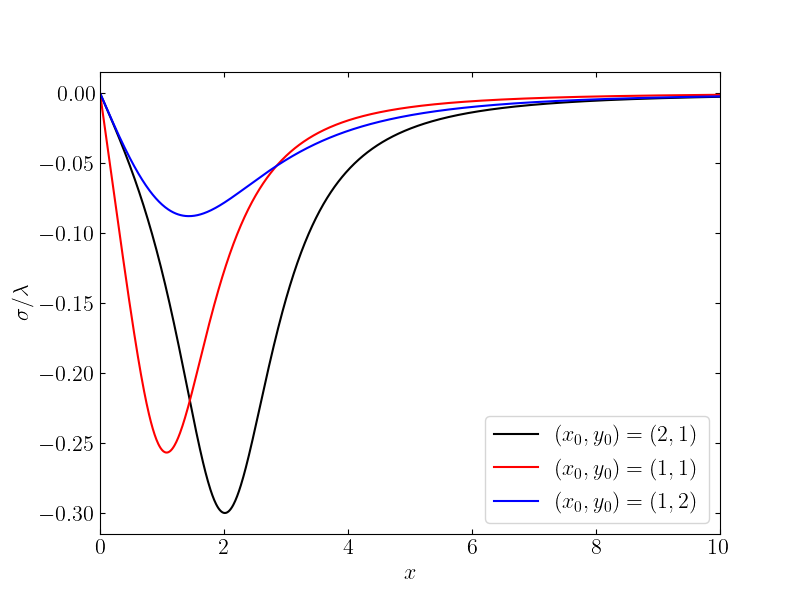
\includegraphics[width=0.9\textwidth]{p3.png} 
    \end{center}

    (c) At the plane $y=0$, write an area element as $da=dx dz$. Thus, from part
    (b), the total charge per unit length in $z$ is
    \begin{align}
        Q_x&=\int_0^\infty \sigma dx \notag\\
           &=\frac{\lambda}{\pi}\eval{\qty[\tan^{-1}\qty(\frac{x+x_0}{y_0})-\tan^{-1}\qty(\frac{x-x_0}{y_0})]}_0^\infty\notag\\
           &=\frac\lambda\pi\qty[\frac{\pi}{2}-\tan^{-1}\qty(\frac{x_0}{y_0})-\frac\pi2-\tan^{-1}\qty(\frac{x_0}{y_0})]\notag\\
           &=-\frac{2\lambda}{\pi}\tan^{-1}\qty(\frac{x_0}{y_0})
    \end{align}

    (d) From \eqref{p3:Phi}, we can perform a transformation to polar coordinate
    $(x,y)=\rho(\cos\theta,\sin\theta)$ and
    $(x_0,y_0)=\rho_0(\cos\theta_0,\sin\theta_0)$ and write
    \begin{align}
        \Phi&=-\frac{\lambda}{4\pi\epsilon_0}\qty[
        \ln\qty(\frac{\rho^2+\rho_0^2-2\rho\rho_0\cos(\theta-\theta_0)}{\rho^2+\rho_0^2-2\rho\rho_0\cos\qty(\theta+\theta_0)})
        +\ln\qty(\frac{\rho^2+\rho_0^2+2\rho\rho_0\cos(\theta-\theta_0)}{\rho^2+\rho_0^2+2\rho\rho_0\cos\qty(\theta+\theta_0)})
        ]\notag\\
            &=-\frac{\lambda}{4\pi\epsilon_0}\qty[
            \ln\qty(\frac{1+\epsilon^2-2\epsilon\cos\qty(\theta-\theta_0)}{1+\epsilon^2-2\epsilon\cos\qty(\theta+\theta_0)})
            +\ln\qty(\frac{1+\epsilon^2+2\epsilon\cos\qty(\theta-\theta_0)}{1+\epsilon^2+2\epsilon\cos\qty(\theta+\theta_0)})
            ]\tag{$\epsilon\equiv\rho_0/\rho$}\\
            &\approx-\frac{\lambda}{4\pi\epsilon_0}\qty[-4\sin(2\theta)\sin(2\theta_0)\epsilon^2+\order{\epsilon^3}]\notag\\
            &\approx\frac{4\lambda}{\pi\epsilon_0}\frac{(\rho\cos\theta)(\rho\sin\theta)(\rho_0\cos\theta_0)(\rho_0\sin\theta_0)}{\rho^4}\notag\\
            &=\frac{4\lambda}{\pi\epsilon_0}\frac{(xy)(x_0y_0)}{\rho^4}
    \end{align}
    where we have assumed $\rho\gg\rho_0$ in the third equality. This
    2D potential
    is quadrupole, which is expected because there are two dipoles (formed by
    the 3 image charges and the real charge).
\end{solution}
\end{problem}
%%%%%%%%%%%%%%%%%%%%%%%%%%%%%%%%%%%%%%%%%%%%%%%%%%%%%%%%%%%%%%%%%%%%%%%%%%%%%%%%
\begin{problem}{3.4}[Green's function in Cartesian coordinates]
(a) Show that the Green function $G(x,y;x',y')$ appropriate for Dirichlet
boundary conditions for a square two-dimensional region, $0\leq x\leq1,0\leq
y\leq1$, has an expansion
\begin{equation}
    G(x,y;x',y')=2\sum_{n=1}^\infty g_n(y,y')\sin(n\pi x)\sin(n\pi x') 
\end{equation}
where $g_n(y,y')$ satisfies
\begin{equation}
    \qty(\frac{\partial^2}{\partial y'^2}-n^2\pi^2)g_n(y,y')
    =-4\pi\delta(y'-y)
    \qquad\text{and}\qquad
    g_n(y,0)=g_n(y,1)=0
\end{equation}

(b) Taking for $g_n(y,y')$ appropriate linear combinations of $\sinh\qty(n\pi
y')$ and $\cosh(n\pi y')$ in the two regions, $y'<y$ and $y'>y$, in accord with
the boundary conditions and the discontinuity in slope required by the source
delta function, show that the explicit form of $G$ is
\begin{equation}
    G(x,y;x',y')=8\sum_{n=1}^\infty
        \frac{1}{n\sinh(n\pi)}\sin(n\pi x)\sin(n\pi x')\sinh(n\pi
        y_<)\sinh\qty[n\pi\qty(1-y_>)]
\end{equation}
where $y_<(y_>)$ is the smaller (larger) of $y$ and $y'$.
\begin{solution}
    (a) First, we expand $G(x,y;x',y')$ in a Fourier series with the
    orthonormal basis $\mathcal{B}=\qty{\sqrt{2}\sin(n\pi x)}_{n=1}^\infty$ on
    the domain $x\in[0,1]$
    \begin{equation}
        G(x,y;x',y')=\sum_{n,n'\in\N}2g_{n,n'}(y,y')\sin(n\pi x)\sin(n'\pi x') 
    \end{equation}
    Taking the Laplacian $\laplacian'G=(\partial^2/\partial
    x'^2+\partial^2/\partial y'^2)G$, we get from the property of Green's
    functions
    \begin{align}\label{p4a:series}
        \sum_{m,m'\in\N}2&\sin(m\pi x)\sin(m'\pi
        x')\qty(\frac{\partial^2}{\partial
        y'^2}-m'^2\pi^2)g_{m,m'}(y,y')\notag\\
        &\qquad=-4\pi\delta(x-x')\delta(y-y')\notag\\
        &\qquad=-4\pi\delta(y-y')\sum_{m\in\N}2\sin(m\pi x)\sin(m\pi x')
    \end{align}
    where the last equality comes from completeness. Now, note that for our 
    choice of basis $\mathcal{B}$,
    \begin{align}
        \braket{\sqrt2\sin(m\pi x)}{\sqrt2\sin(n\pi x)}
        =\int_0^12\sin(m\pi x)\sin(n\pi x)dx
        =\delta_{m,n}
    \end{align} 
    Thus, taking the inner product of both sides of \eqref{p4a:series} with
    $\sin(n\pi x)$, we get
    \begin{equation}\label{p4a:LHS}
        \braket{\text{LHS}}{\sqrt2\sin(n\pi x)}
        =\sum_{m'\in\N}\sqrt2\sin(m'\pi x')\qty(\frac{\partial^2}{\partial
    y'^2}-m'^2\pi^2)g_{n,m'}(y,y')
    \end{equation}
    and
    \begin{equation}\label{p4a:RHS}
        \braket{\text{RHS}}{\sqrt2\sin(n \pi x)}=-4\pi\delta(y-y')\sqrt2\sin(n \pi x')
    \end{equation}
    Taking the inner product of both sides \eqref{p4a:LHS} and \eqref{p4a:RHS}
    again with $\sqrt2\sin(n\pi x')$, we get
    \begin{equation}\label{p4a:gn}
        \qty(\frac{\partial^2}{\partial
        y'^2}-n^2\pi^2)g_n(y,y')=-4\pi\delta(y-y') 
    \end{equation}
    Thus, $g_n$ has to satisfy \eqref{p4a:gn}. Then the Green function can be
    written as
    \begin{equation}\label{p4a:G}
        G(x,y;x',y')=2\sum_{n\in\N}g_n(y,y')\sin(n\pi x)\sin(n\pi x') 
    \end{equation}
    This obviously vanishes at $x'=0$ and $x'=1$ because $\sin(0)=\sin(n\pi)=0$ 
    for $n\in\N$. But we also have to require that $g_n(y,0)=g_n(y,1)=0$ so that
    $G$ vanishes at $y'=0$ and $y'=1$.

    (b) First, we write
    \begin{equation}
        g_n(y,y')=\begin{cases}
            A_n\sinh(n\pi y')+B_n\cosh(n\pi y') & y'<y\\   
            C_n\sinh(n\pi y')+D_n\cosh(n\pi y') & y'>y
        \end{cases}
    \end{equation}
    For $y\in(0,1)$, $g_n(y,0)=B_n$. Thus we must require that $B_n=0$ due to
    boundary conditions. Similarly, $g_n(y,1)=C_n\sinh(n\pi)+D_n\cosh(n\pi)=0$. Thus
    we can write
    \begin{equation}\label{p4b:gn}
         g_n(y,y')=\begin{cases}
            A_n\sinh(n\pi y')& y'<y\\   
            C_n\qty[\sinh(n\pi y')-\tanh(n\pi)\cosh(n\pi y')] & y'>y
        \end{cases}       
    \end{equation}
    By continuity at $y'=y$, we must require that $\lim_{y'\to
    y^-}g_n=\lim_{y'\to y^+}g_n$, which leads to
    \begin{equation}\label{p4b:A}
        A_n=C_n\qty[1-\frac{\tanh(n\pi)}{\tanh(n\pi y)}] 
    \end{equation}

    Now, from the condition \eqref{p4a:gn}, we can integrate both sides with
    respect to $y'$ in a small region ($y-\epsilon,y+\epsilon$) around $y$ and 
    get
    \begin{equation}
        \eval{\frac{\partial g_n}{\partial y'}}_{y-\epsilon}^{y+\epsilon}
        =n^2\pi^2\int_{y-\epsilon}^{y+\epsilon}g_n(y,y')dy'-4\pi
    \end{equation}
    The integral $I=\int_{y-\epsilon}^{y+\epsilon}g_ndy'$ in the RHS is
    \begin{align}
        I
        &=A_n\int_{y-\epsilon}^y\sinh(n\pi
        y')dy'+C_n\int_y^{y+\epsilon}\qty[\sinh(n\pi y')-\tanh(n\pi)\cosh(n\pi
        y')]dy'\notag\\
        &=\frac{A_n}{n\pi}\qty[\cosh(n\pi y)-\cosh[n\pi(y-\epsilon)]]\notag\\
        &\qquad+\frac{C_n\tanh(n\pi)}{n\pi}\qty[\cosh[n\pi(y+\epsilon)]-\cosh(n\pi
        y)+\sinh(n\pi y)-\sinh[n\pi(y+\epsilon)]]
    \end{align}
    As $\epsilon\to0$, $I\to0$. So the jump condition is
    \begin{align}
        -4\pi=\eval{\frac{\partial g_n}{\partial
        y'}}_{y'=y+\epsilon}-\eval{\frac{\partial g_n}{\partial
y'}}_{y'=y-\epsilon}
        &=C_nn\pi\qty[\cosh[n\pi(y+\epsilon)]-\tanh(n\pi)\sinh[n\pi(y+\epsilon)]]\notag\\
        &\qquad-A_nn\pi\cosh[n\pi(y-\epsilon)]
    \end{align}
    As $\epsilon\to0$, we can use \eqref{p4b:A} and write from the jump
    condition
    \begin{equation}
        C_n=-\frac{4}{n}\frac{\sinh(n\pi y)\cosh(n\pi)}{\sinh(n\pi)}
    \end{equation}
    It also follows that
    \begin{equation}
        A_n=-\frac4{n}\frac{\sinh(n\pi
        y)}{\tanh(n\pi)}\qty[1-\frac{\tanh(n\pi)}{\tanh(n\pi y)}]
        =-\frac{4}{n}\frac{\sinh[n\pi(y-1)]}{\sinh(n\pi)}
    \end{equation}
    Plugging these back into \eqref{p4b:gn}, we get
    \begin{align}
        g_n&=\begin{cases}
            \frac{4}{n\sinh(n\pi)}\sinh(n\pi y')\sinh[n\pi(1-y)] & y'<y\\
            \frac{4}{n\sinh(n\pi)}\sinh(n\pi y)\sinh[n\pi(1-y')] & y'>y
        \end{cases}\notag\\
           &=\frac4{n\sinh(n\pi)}\sinh(n\pi y_<)\sinh[n\pi(1-y_>)]
    \end{align}
    where $y_<=\min(y,y')$ and $y_>=\max(y,y')$. Then the Green function
    \eqref{p4a:G} can be written as
    \begin{equation}
        G(x,y;x',y')=8\sum_{n\in\N}\frac{1}{n\sinh(n\pi)}\sinh(n\pi
        y_<)\sinh[n\pi(1-y_>)]\sin(n\pi x)\sin(n\pi x') 
    \end{equation}
    as desired.
\end{solution}
\end{problem}
%%%%%%%%%%%%%%%%%%%%%%%%%%%%%%%%%%%%%%%%%%%%%%%%%%%%%%%%%%%%%%%%%%%%%%%%%%%%%%%%

\end{document}
